\documentclass{beamer}


\usepackage{amsmath}
\usepackage{listings}
\usepackage{color}
\usepackage{verbatim}
\definecolor{codegreen}{rgb}{0,0.6,0}

\lstset{ %
  basicstyle=\fontsize{11}{11}\ttfamily,
  backgroundcolor=\color{white},   % choose the background color; you must add \usepackage{color} or \usepackage{xcolor}; should come as last argument
  breakatwhitespace=false,         % sets if automatic breaks should only happen at whitespace
  captionpos=b,                    % sets the caption-position to bottom
  commentstyle=\color{codegreen},    % comment style
  keepspaces=true,                 % keeps spaces in text, useful for keeping indentation of code (possibly needs columns=flexible)
  rulecolor=\color{black},         % if not set, the frame-color may be changed on line-breaks within not-black text (e.g. comments (green here))
  showspaces=false,                % show spaces everywhere adding particular underscores; it overrides 'showstringspaces'
  showstringspaces=false,          % underline spaces within strings only
  showtabs=false,                  % show tabs within strings adding particular underscores
  tabsize=2,	                     % sets default tabsize to 2 spaces
}





\mode<presentation> {

% The Beamer class comes with a number of default slide themes
% which change the colors and layouts of slides. Below this is a list
% of all the themes, uncomment each in turn to see what they look like.

%\usetheme{default}
%\usetheme{AnnArbor}
%\usetheme{Antibes}
%\usetheme{Bergen}
%\usetheme{Berkeley}
%\usetheme{Berlin}
%\usetheme{Boadilla}
%\usetheme{CambridgeUS}
%\usetheme{Copenhagen}
%\usetheme{Darmstadt}
%\usetheme{Dresden}
%\usetheme{Frankfurt}
%\usetheme{Goettingen}
%\usetheme{Hannover}
%\usetheme{Ilmenau}
%\usetheme{JuanLesPins}
%\usetheme{Luebeck}
\usetheme{Madrid}
%\usetheme{Malmoe}
%\usetheme{Marburg}
%\usetheme{Montpellier}
%\usetheme{PaloAlto}
%\usetheme{Pittsburgh}
%\usetheme{Rochester}
%\usetheme{Singapore}
%\usetheme{Szeged}
%\usetheme{Warsaw}

% As well as themes, the Beamer class has a number of color themes
% for any slide theme. Uncomment each of these in turn to see how it
% changes the colors of your current slide theme.

%\usecolortheme{albatross}
%\usecolortheme{beaver}
%\usecolortheme{beetle}
%\usecolortheme{crane}
%\usecolortheme{dolphin}
%\usecolortheme{dove}
%\usecolortheme{fly}
%\usecolortheme{lily}
%\usecolortheme{orchid}
%\usecolortheme{rose}
%\usecolortheme{seagull}
%\usecolortheme{seahorse}
%\usecolortheme{whale}
%\usecolortheme{wolverine}

%\setbeamertemplate{footline} % To remove the footer line in all slides uncomment this line
%\setbeamertemplate{footline}[page number] % To replace the footer line in all slides with a simple slide count uncomment this line

%\setbeamertemplate{navigation symbols}{} % To remove the navigation symbols from the bottom of all slides uncomment this line
}

\usepackage{graphicx} % Allows including images
\usepackage{booktabs} % Allows the use of \toprule, \midrule and \bottomrule in tables

%----------------------------------------------------------------------------------------
%	TITLE PAGE
%----------------------------------------------------------------------------------------

\title[]{
\Large{Approximations to the distribution\\ of a large quadratic form}
} % The short title appears at the bottom of every slide, the full title is only on the title page
\institute[]{Department of Statistics\\University of Auckland}
\author{Tong Chen \and Thomas Lumley}



\date{NZSA, 2018} % Date, can be changed to a custom date

\begin{document}

\begin{frame}
\titlepage % Print the title page as the first slide
\end{frame}


%----------------------------------------------------------------------------------------
%	PRESENTATION SLIDES
%----------------------------------------------------------------------------------------

\section{Introduction}
%------------------------------------------------

\begin{frame}{What is a quadratic form?}
\begin{center}
  \begin{itemize}
  \item{If $X$ is an $n$ dimensional vector with mean vector $\mu$ and covariance matrix $\Sigma$. A quadratic form in $\mathbb{R}$ is a function of ${Q(X)}$: $\mathbb{R}^n \to \mathbb{R}$, which could be expressed as:
	\[ Q(X) = X^{T}AX\]
	where $A$ is an $n \times n$ symmetric and non-negative definite matrix..}
  \bigskip
  \item The question of interest is to estimate $Pr(Q(X)>q)$.
  \end{itemize}
\end{center}
\end{frame}

%------------------------------------------------

%------------------------------------------------

\begin{frame}{Why is it interesting?}
\begin{center}
  \begin{itemize}
   \item The distribution of $Q(X)$ is a linear combination of noncentral $\chi_1^2$ variables.
   \bigskip
  
   \item These quadratic forms are used when a set of asymptotically Normal test statistics
are combined using a weight matrix other than the inverse of their covariance matrix.
   \bigskip
   
   \item{ Null distribution: a quadratic form in Gaussian variables\\
   \begin{center}
   $Q(X) = X^TAX = Y^T\Lambda Y =\sum \lambda_i \chi^2_1$
   \end{center}
   where $\lambda_1 \dots \lambda_n$ are the eigenvalues of $\Sigma A$.
  }
  \end{itemize}
\end{center}
\end{frame}
%------------------------------------------------
\begin{frame}{Large quadratic forms in genetics studies}
 \begin{itemize}
   \item Previous study mainly focused on 
   \begin{enumerate}
      \item small quadratic forms $(n < 10)$
      \item large p-value $(p > 10^{-2})$
   \end{enumerate}
   \bigskip
   \item In genetics studies, we have 
   \begin{enumerate}
      \item large quadratic forms $(n > 1000)$
      \item very small p-value $(p < 10^{-4})$
   \end{enumerate}
   \bigskip
   \item Existing methods may have problems in both accuracy and computational time.
   \end{itemize}
\end{frame}

%------------------------------------------------
\begin{frame}{Existing methods}
 \begin{itemize}
    \item `Exact' methods: the approximation error can be arbitrarily small if calculations are done to arbitrary precision. 
    \bigskip
    \item Approximations based on matching moments 
    \bigskip
    \item A saddlepoint approximation
    
   \end{itemize}
\end{frame}

%------------------------------------------------
\begin{frame}{`Exact' methods}
 \begin{itemize}
    \item Davies (1980) approximated the distribution of $Q(X)$ based on the characteristic function of $Q(X)$.
    \bigskip
    \item Farebrother (1984) wrote $Pr(Q(X)>q)$ as an infinite series of central chi-square distribution. This is done by writing the linear combination as a mixture (Robbins and Pitman, 1949).
    \bigskip
    \item Bausch (2013) showed that a linear combination of gamma
densities form an algebra under convolution.
   \end{itemize}
\end{frame}


%------------------------------------------------
\begin{frame}{Moment based methods}
 \begin{itemize}
   \item Liu et al. (2009) (four-moment approximation):
    \begin{enumerate}
    \item Using $\chi_l^2(\delta)$ to approximate $Q(x)$
    \item $l$ and $\delta$ are obtained by equalling the skewnesses and minimizing the difference between kurtosis of $Q(x)$ and $\chi_l^2(\delta)$.
    \end{enumerate}
    \bigskip
   \item Satterthwaite approximation:
   \begin{enumerate}
    \item Using $a\chi_v^2$ to approximate $Q(x)$.
    \begin{flalign*}  
a = (\sum_{i=1}^{n} \lambda_i^2)/ (\sum_{i=1}^{n} \lambda_i) \hspace{15pt}
v = (\sum_{i=1}^{n} \lambda_i) ^2/(\sum_{i=1}^{n} \lambda_i^2).
\end{flalign*}
    \item Give correct mean and variance
    \item $\sum \lambda =$ trace$(\Sigma A)$ and $\sum \lambda^2 =$ trace$((\Sigma A)^2) = \sum_{i,j} a_{i,j}^2$. Thus they are available in $O(n^2)$ time.  
    \end{enumerate}
   \end{itemize}
\end{frame}


%------------------------------------------------
\begin{frame}{A saddlepoint approximation}
 \begin{itemize}
 \item Kuonen (1999) proposed a form of saddlepoint approximation based on a Normal approximation to an exponentially-shifted density.
 \bigskip
 \item To obtain $Pr(X>z)$ for a density $f_X(x)$, create an exponential family $g(x;\theta) = cf(x)\exp(x\theta)$. Then choosing $\theta$ so that $z$ is the mean of density $g(x;\theta)$ (Normal approximation to the sum works well near the mean).
 \bigskip
 \item It's known that the first-order term in the error is uniformly bounded. 
   \end{itemize}
\end{frame}



%------------------------------------------------

\begin{frame}{Accuracy - the distribution of $Q(X)$}
\begin{lemma}\label{aa}
$Pr(\sum \lambda_i z_i^2 >q) \simeq ce^{-\frac{1}{2\lambda_1} q}$ for large $q$.
\end{lemma}
\begin{itemize}
\bigskip
\item The density for $\chi_k^2$ is
\begin{flalign*}
f(x) = \frac{x^{\frac{k}{2}-1}e^{-\frac{x}{2}}}{2^{\frac{k}{2}}\Gamma(\frac{k}{2})} 
\end{flalign*}
When $x$ is big, only exponential matters.
\bigskip
\item If $X$ and $Y$ have exponential tails with different tail rates, $X+Y$ has an exponential tail and tail rate is dominated by the one with larger multiplier (Berman et al., 1992). 
\end{itemize}
\end{frame}


%------------------------------------------------
\begin{frame}{Accuracy - Exact methods}
\begin{itemize}
    \item Davies's and Farebrother's method would break down when p-value is close to or beyond machine epsilon
    \bigskip
    \item They compute $1-(1-Pr(Q>q))$
\end{itemize}
\begin{figure}[H]	 
	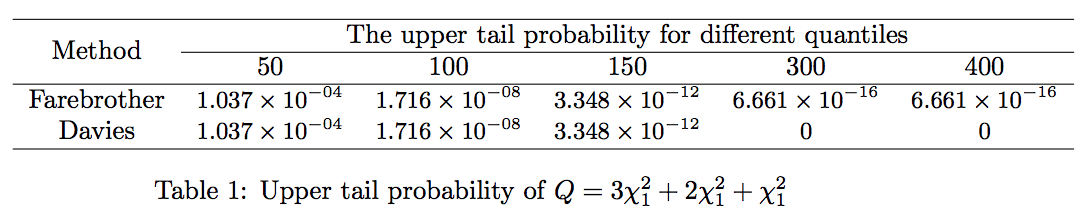
\includegraphics[scale = 0.6]{plot4.png}
\end{figure} 
\end{frame}

%------------------------------------------------
\begin{frame}{Accuracy - Exact methods}
\begin{itemize}
    \item Farebrother's method is not usable if the smallest eigenvalue is much smaller than the leading terms for large $n$. Because it would cause $a_0$ in the algorithm to underflow.
    \begin{flalign*}
     a_0 = exp\left(\frac{1}{2}(n\log \lambda_n - \sum_i^n \log \lambda_i) \right)
    \end{flalign*}
    \bigskip
    \item Bausch's method has rounding error especially in the left tail with double precision and is slow with multiple precision.
\end{itemize}
\end{frame}

%------------------------------------------------

\begin{frame}{Accuracy}
\begin{itemize}
\item Moment methods approximate the distribution of $Q(X)$ with a single $\chi_k^2$. They are anti-conservative in extreme tails.

\bigskip

\item The saddlepoint approximation has the correct exponential tail rate in the extreme right tail. 
\end{itemize}
\end{frame}

%------------------------------------------------

\begin{frame}{Time complexity}
\begin{itemize}
    \item Finding all the eigenvalues are slow for large $n$.
    \bigskip
    \item Computing all $\lambda$, the time complexity is $O(n^3)$.
    \bigskip
    \item Computing the leading $k$ $\lambda_i$, the time complexity is $O(kn^2)$
\end{itemize}
\end{frame}
%------------------------------------------------
\begin{frame}{A leading eigenvalue approximation}
\begin{center}
\begin{itemize}
  \item Lumley et al. (2018) proposed a leading eigenvalue approximation
  \begin{enumerate}
  \item Only compute the largest $k$ eigenvalues
    \begin{enumerate}
    \item using Subsampled Random Hadamard Transform (Tropp, 2011) to get a linear transformed $H$.
    \item use the QR decomposition to the matrix $(H\Sigma A)^T$ to get an orthonormal matrix $Q$.
    \item the eigenvalue decomposition of $Q \Sigma A Q^T$
    \end{enumerate}

  \item Using Satterthwaite approximation to approximate the rest
  \end{enumerate}
  \bigskip
  \item The reference distribution is
          \begin{flalign*}
 \small{T \sim \Big( \sum_{i=1}^{k} \lambda_i  \chi_1^2 \Big) + a \chi_{v}^2}
\end{flalign*} 
where $\lambda_1,...,\lambda_k$ are the largest $k$ eigenvalues of $\Sigma A$.
\end{itemize}
\end{center}
\end{frame}
%------------------------------------------------

\begin{frame}{A leading eigenvalue approximation}
\begin{center}
\begin{itemize}
  \item The time complexity is $O(kn^2)$
  \begin{enumerate}
    \item Compute the largest $k$ eigenvalues using random matrix theory.
    \item Remainder term is available in $O(n^2)$ time.
  \end{enumerate}
  \bigskip
  \item Accuracy: the tail rate is correct.
  \bigskip
  \item Approximate $Q(X)$ with leading terms using:
  \begin{enumerate}
  \item exact method when p-value ranges from $10^{-13}$ to $1$
  \item the saddlepoint approximation when p-value ranges from $0$ to $10^{-13}$.
  \end{enumerate}
\end{itemize}
\end{center}
\end{frame}

%------------------------------------------------

\begin{frame}{Data generation}
\begin{itemize}
\item Using the Markov Coalescent simulator (Chen et al., 2009) 
\begin{enumerate}
    \item fix $n$ to obtain $m \approx n$
    \item discard variants if minor allele frequency $>5\%$
    \item result in a large sparse matrix
\end{enumerate}
\bigskip
\item Generate 5 datasets:
\end{itemize}
\begin{figure}[H]	 
	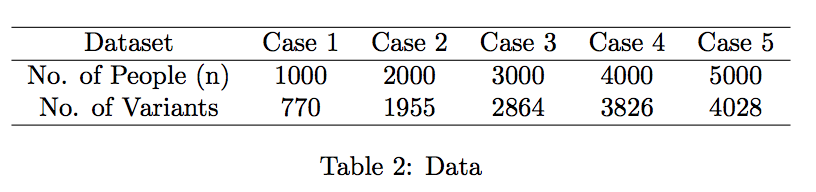
\includegraphics[scale = 0.7]{plot2.png}
\end{figure} 
\end{frame}


%------------------------------------------------
\begin{frame}{Empirical comparisons}
\begin{itemize}
\item Compare a leading eigenvalue approximation with a full eigendecomposition of Davies's method. 
\end{itemize}
\begin{figure}[H]	 
	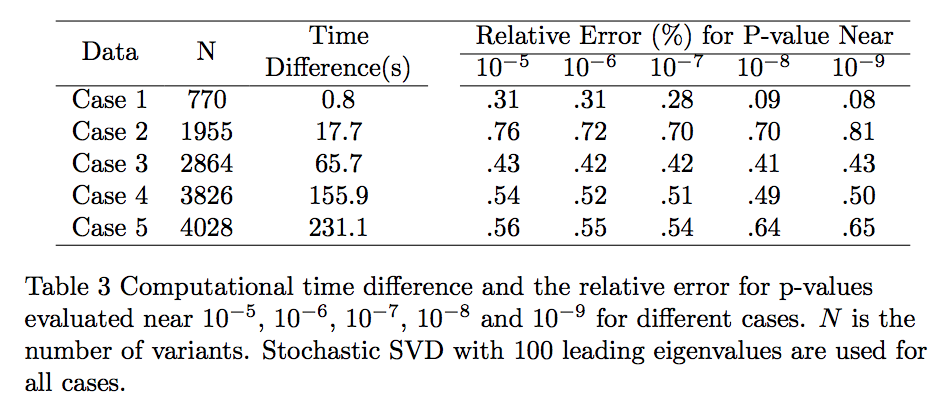
\includegraphics[scale = 0.65]{plot3}
\end{figure}    
\end{frame}

%------------------------------------------------
\begin{frame}{Comparing versions of a leading eigenvalue approximation}
\begin{itemize}
    \item Remainder term 1: approximated by Satterthwaite approximation
    \bigskip
    \item \color{red}Remainder term 2: aprroximated by matching the mean.
    \bigskip
    \item \color{blue} Version 3: has no remainder term
\end{itemize}
\end{frame}

%------------------------------------------------
\begin{frame}{Comparing versions of a leading eigenvalue approximation}
\begin{figure}[H]	 
	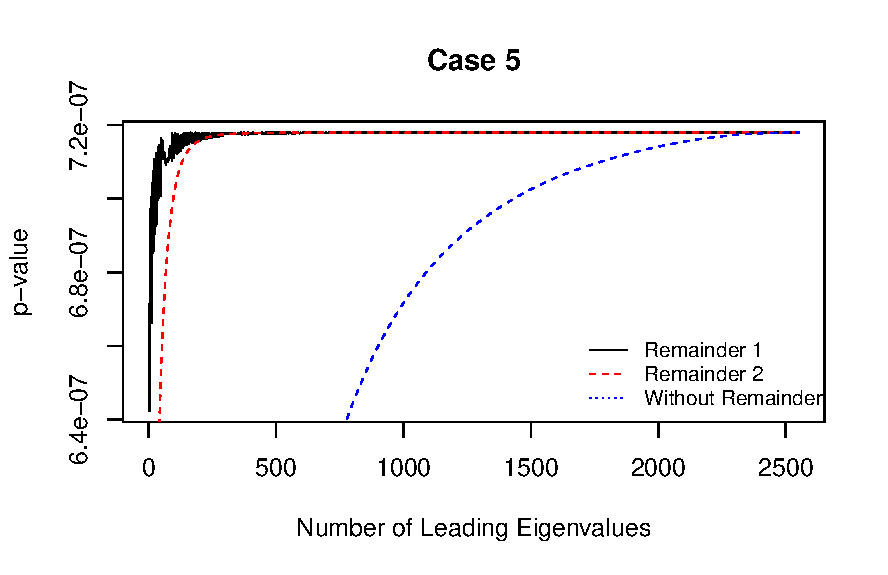
\includegraphics[scale = 0.6]{Rplot15.pdf}
\end{figure} 
\begin{itemize}
    \item The version with remainder term using the Satterthwaite approximation is not very sensitive to the choice of $k$.
\end{itemize}
\end{frame}

\begin{frame}{Extreme tail comparisons}
\begin{itemize}
    \item Comparisons of a leading eigenvalue approximation with Davies's method (left panel) and the saddlepoint approximation (right panel).
\end{itemize}
\begin{figure}[H]	 
 	\begin{subfigure}
 		\centering
 		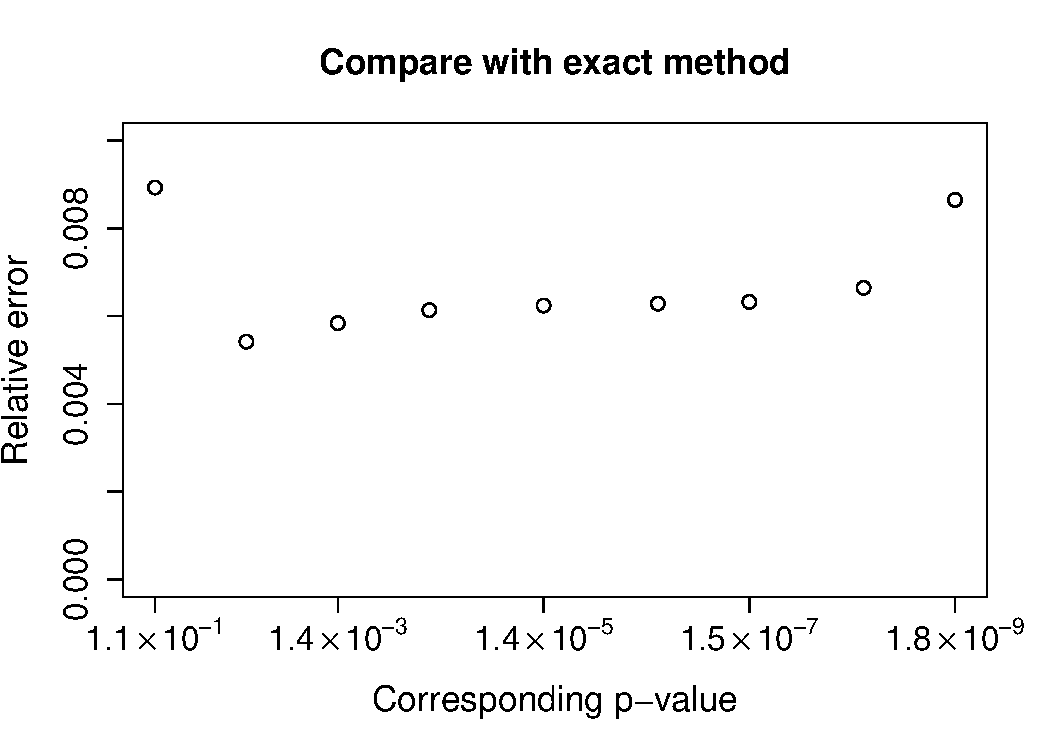
\includegraphics[width=0.45\linewidth]{Rplots5.pdf}
 	\end{subfigure}	
 	\begin{subfigure}
 		\centering
 		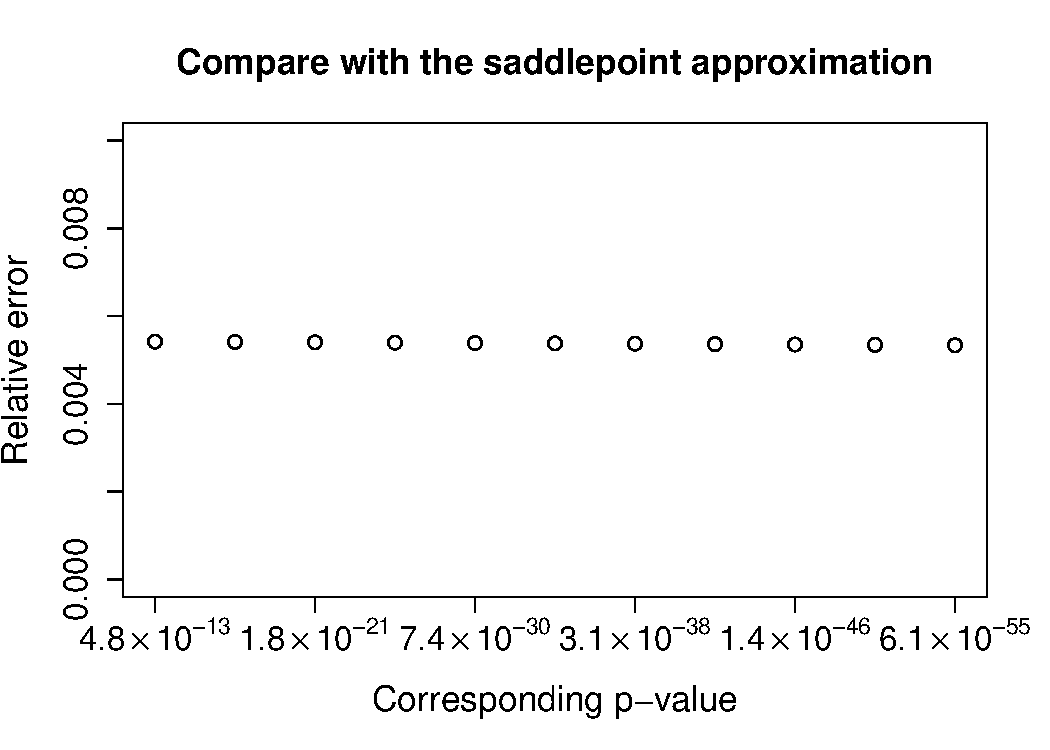
\includegraphics[width=0.45\linewidth]{Rplots6.pdf}
 	\end{subfigure}	
 \end{figure}    
\end{frame}
%------------------------------------------------

\begin{frame}{Recommendation}
\begin{itemize}
    \item If $n > 1000$ and p-value $> 10^{-13}$, a leading eigenvalue approximation combined with Davies's method is optimal.
    \bigskip
    \item If $n > 1000$ and p-value $< 10^{-13}$, a leading eigenvalue approximation combined with the saddlepoint approximation is optimal.
    \bigskip
    \item If $n < 1000$ and p-value $> 10^{-13}$, a full eigendecomposition of Davies's method is optimal.
    \bigskip
    \item If $n < 1000$ and p-value $< 10^{-13}$, a full eigendecomposition of the saddlepoint approximation is optimal.
\end{itemize}
    \end{frame}
%------------------------------------------------
\begin{frame}[fragile]

\begin{center}
\Huge Thank You!
\end{center}


\end{frame}

\end{document}
